\documentclass[twoside]{article}
\usepackage{aistats2015}
\usepackage{graphicx}
\usepackage{pgfplots}
\usepackage{float}
\usepackage{subfig}
\usepackage{hyperref}
\usepackage{natbib}
\usepackage{amsmath}

\bibpunct{[}{]}{;}{n}{,}{,}

\usetikzlibrary{external} \tikzexternalize[prefix=figures/precompiled/]

    \newlength\figureheight \newlength\figurewidth

\begin{document}

\twocolumn[

\aistatstitle{Learning to Control Kilobots with a Flashlight}
\aistatsauthor{Alexander Hendrich \And Daniel Kauth \And Gregor Gebhardt}
\aistatsaddress{TU Darmstadt \And TU Darmstadt \And TU Darmstadt}]

\begin{abstract}
The recently emerged kilobots provide lots of new applications for swarm
intelligence and collective behavior algorithms. By applying a light following
behavior called \emph{Phototaxis} to the kilobots, they provide an easy method
to move and control large quantities at the same time. By interacting with the
lightsource(s) (switching them on/off or moving a single light source) a human
can control a kilobot swarm to fulfill certain tasks, for example pushing an
object through a maze\cite{kilobotMaze}. In this project we want to learn to
control the light to achieve this behavior.
\end{abstract}

\section{INTRODUCTION}

Our task is to learn to push an object through a maze with a swarm of kilobots
by moving a single light source. Because this task is quite complex and
difficult to learn, we split it up into two separate problems with two separate
policies.

The first problem is to find an optimal path through the labyrinth.
The policy should return a movement direction for each possible object position.
By constantly following these movements, the object should reach the goal
position independent of its starting position.

Because we cannot directly
control the object's movement we need a method to interact with the light
source, so that the kilobots push the object in the desired direction. This will
be the focus of the second problem. The policy should return a new light
position depending on the output of the first policy (the desired movement
direction of the object) and the relative position of the kilobots towards the
object.

\begin{figure}[!htb] \centering
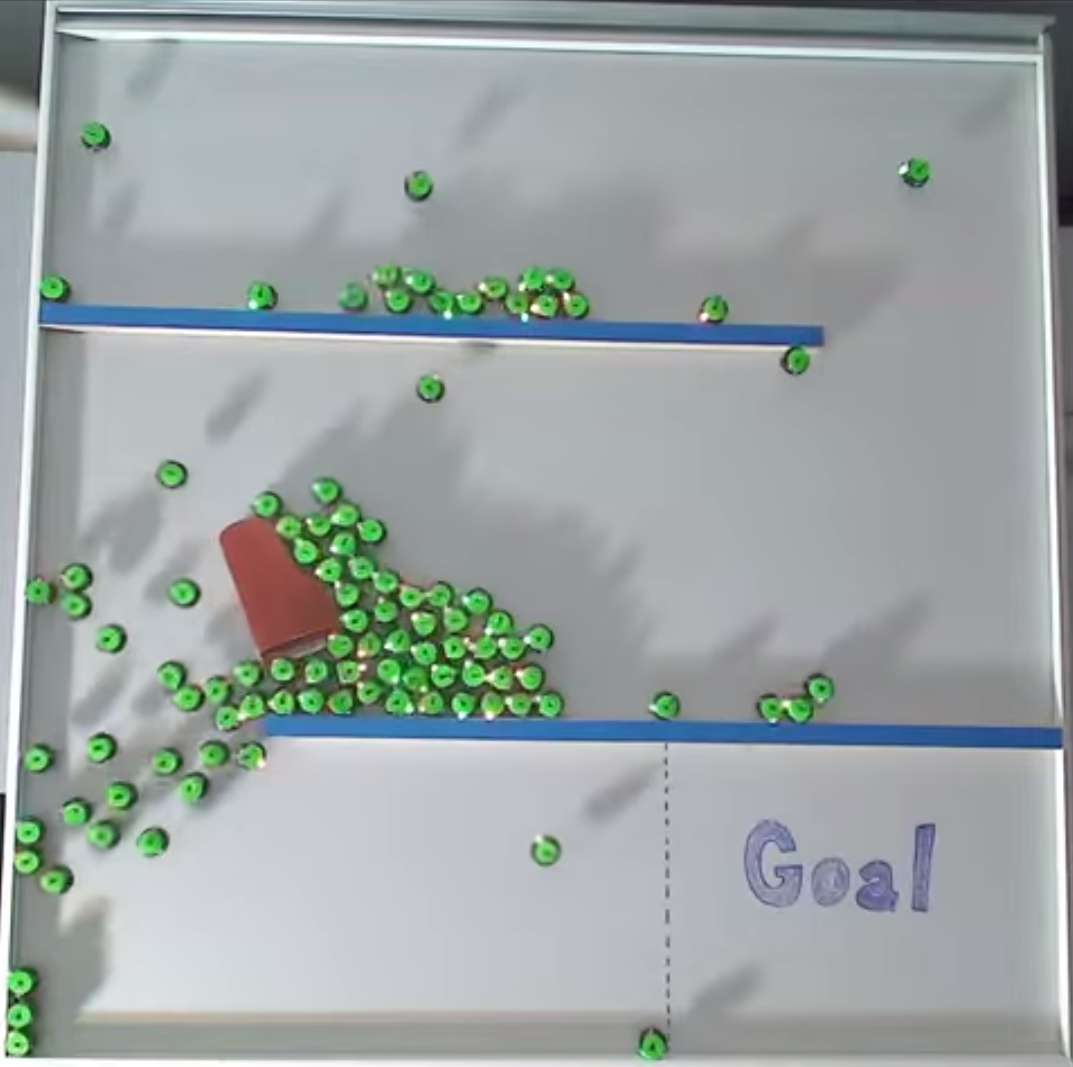
\includegraphics[width=0.8\linewidth]{figures/inspiration.png} \caption{Kilobots
pushing a small object through a maze by human controlled light sources}
\end{figure}

\section{PRELIMINARIES} In the following sections we introduce our used
materials (kilobots\cite{kilobot}) and methods (Actor Critic Relative Entropy
Policy Search)\cite{acreps}.

\subsection{Kilobots} Kilobots\cite{kilobot} are open-source, low cost robots
specially designed to explore collective algorithms and decentralized
cooperation. With previous robots these methods could only be tested in a
simulator or in small quantities of robots because acquiring and controlling
hundreds or even thousands of them is very cost-intensive, time consuming and
complex. To eliminate this issue Harvard University developed Kilobots. Each
robot is made with only 14\$ worth of parts and large collectives can easily be
controlled by a single user.

The low cost however results in limited capabilities of each individual robot.
For example, the kilobot doesn't use complex steering or wheels for locomotion.
Instead it stands on three solid legs and moves by activating two small
vibrating motors placed on each side of the kilobot. This form of movement only
allows for very low movement speeds of up to 1cm per second and can only be
performed on special surfaces (e.g. glass).

To communicate with each other, each kilobot has an infrared transmitter and
receiver on the bottom. Messages are passed by emitting infrared light onto the
reflecting glass and can be received by another kilobot up to 7-10cm away
(radius of each kilobot is 3.3cm). By measuring the received signal strength,
the kilobots are capable of estimating their distances to each other.

The kilobot also possesses an ambient light sensor to determine the light
intensity at its current location. Depending on the current and previously
measured light intensity the robot alternates between left and right turns to
move towards the light source. This behavior is called \emph{Phototaxis} and is
used to control a whole swarm of robots at once. While performing left or right
turns the robot only activates one of its two motors and the robot doesn't move
in a straight line, which further reduces its movement speed.

\begin{figure}[!htb] \centering
    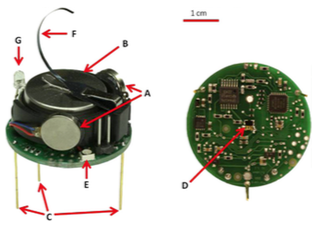
\includegraphics[width=0.9\linewidth]{figures/kilobot.png}
    \caption{Isometric (left) and bottom (right) views of a Kilobot. Some key
    features are: (A) vibration motors, (B) lithium-ion battery, (C) rigid
supporting legs, (D) infrared transmitter/receiver, (E) three-color (RGB) LED,
(F) charging tab, and (G) ambient light sensor. Note the 1 cm line for
scale.\cite{kilobot}} \end{figure}

\subsection{Actor Critic Relative Entropy Policy Search}
\emph{Actor critic relative entropy policy search} (AC-REPS) as introduced by
\cite{acreps} is a method for policy improvement based on \emph{relative entropy
policy search} (REPS) \cite{reps} which allows for model-free learning with
non-parametric continous policies and random exploration. It consists of the
following three steps:

\subsubsection{Estimating the Q-Function}
During the simulation we generate sample in the form $(s_i, a_i, r_i, s'_i)$,
where we start in state $s_i$, take action $a_i$ to get to state $s'_i$ and
get reward $r_i$. We also define a feature-based Q-function as $Q(s, a) =
\phi(s,a)^T \theta$ with feature function $\phi(s,a)$ and parameter vector
$\theta$. Details of our state and action representations and rewards and
features we used are discussed in section TODO.

To estimate $\theta$ we use \emph{Least-squares temporal difference
learning} (LSTD) with $L_{22}-Regularization$\cite{lstdRegularization} as
follows:

With $n$ being the number of sample and $k$ being the number of features
we define the two feature matrices $\Phi$ and $\Phi'$ (size $n\times k$)
$$
\Phi = \left(
\begin{array}{c}
    \phi(s_1,a_1)^T \\
    \phi(s_2,a_2)^T \\
    \dots \\
    \phi(s_n,a_n^T)
\end{array} \right), \;
\Phi' = \left(
\begin{array}{c}
    \mathbf{E}_{\pi(a_1'|s_1')} [\phi(s_1', a_1') | s_1']^T \\
    \mathbf{E}_{\pi(a_2'|s_2')} [\phi(s_2', a_2') | s_2']^T \\
    \dots \\
    \mathbf{E}_{\pi(a_n'|s_n')} [\phi(s_n', a_n') | s_n']^T \\
\end{array} \right)
$$
and the reward vector
$$
R = \left(
\begin{array}{c}
    r(s_1) \\
    r(s_2) \\
    \dots \\
    r(s_n)
\end{array} \right).
$$
For $\Phi'$ we estimate the expected value
$$
\mathbf{E}_{\pi(a_i'|s_i')} [\phi(s_i', a_i') | s_i']
$$
by taking the average over $p$ samples $a_i' \sim \pi(a_i'|s_i')$, where $\pi$
is our current policy.

Using the derivations of \cite{lspi} and \cite{lstdRegularization} we can easily
compute $\theta$ as
$$
\theta = (X^TX+\beta'I)^{-1}X^Ty
$$
with
$$X = C(A+\beta I) \qquad y=Cb$$
$$A = \Phi^T(\phi-\gamma \Phi') \qquad b=\Phi^T R$$
$$C = \Phi(\Phi^T\Phi+\beta I)^{-1},$$
where $\beta$ and $\beta'$ are regularization parameters for the projection and
fixed-point step, which make the estimation numerically more stable and improve
noise tolerance.

\subsubsection{Actor Critic REPS}
In this step we find a new policy $\pi'$ which optimizes the expected Q-value
as given by our estimated Q-function, but has a limited Kullback-Leibner (KL)
distance to the old policy $\pi$.

To achieve this we optimize over the joint state action distribution
$p(s,a) = p(s) \pi'(s, a)$ and require that the estimated state distribution
$p(s)$ is the same as in the given state sample distribution $\mu(s)$.
This is implemented by matching feature averages of $p(s)$ and $\mu(s)$ and
leads to the following optimization problem:
\begin{align}
    & \max_p \int p(s, a)Q(s, a)\:ds\:da\:, \\
    & \text{s.t. } \text{KL}(p(s, a) || \mu(s)\pi(a|s)) \leq \epsilon,\\
    & \int p(s)\phi(s)\:ds = \hat{\phi}, \int p(s, a)\:ds\:da = 1,
\end{align}
where $\hat{\phi} = \int p(s) \phi(s)\:ds$ is the average feature vector of all
state samples and $\phi(s)$ is another feature function.

This problem can be solved using Lagrangian multipliers and has the solution
$$
p(s)\pi'(a|s) \propto \mu(s) \pi(a|s) \exp\left(\frac{Q(s,a) - V(s)}{\eta}\right),
$$
where $V(s) = v^T \phi(s)$ and $\eta$ and $v$ are Lagrangian multipliers which
can be obtained by minimizing the dual function using standard gradient methods.

\subsubsection{Obtaining a new Policy}
Lastly we need to fit a new policy to our desired probabilities
$p(s_i, a_i) = p(s_i) \pi'(a_i|s_i)$. This is done by minimizing the KL
divergence between $\pi'$ and our new policy $\bar{\pi}$ which is equivalent to
computing a weighted maximum likelihood estimate with sample weights
$$
w_i = \exp\left(\frac{Q(s_i, a_i) - V(s_i)}{\eta}\right).
$$

In this paper we use a weighted Sparse Gaussian Process to obtain our new policy
$\bar{\pi}$. TODO citation / explain Sparse GP?

\section{LEARNING PROCESS}

\subsection{Object Pushing Policy}

\subsection{Maze solving Policy}

TODO use maze solver or just points list?

\section{FUTURE WORK \& CONCLUSION} Our goal for the second part of this project
is to learn how to control the kilobots, so that they can push a given object
(e.g. flat cylinder) towards the desired direction given by our first policy. To
achieve this goal, the policy first has to move the kilobots behind the object.
Depending on the shape of the object (flat cylinder compared to an ``L''-shaped
object), the optimal positions for the kilobots to push can be different if the
object is rotated.

Our initial approach was to solve the two problems at once, so we already went
through some attempts to model the pushing behavior. Although we could not
achieve satisfactorily results with this approach, we feel confident that our
modeling will return good results once we split up the problem into two distinct
problems. To model the pushing behavior we need to find a good position behind
the object and then push the object with the kilobots. Therefore we placed two
rings of RBFs around the object's position. Because we split up the two policies
we can also increase the number of RBFs we used for the pushing behavior or even
spread them on a grid around the object.

Because we want to apply our learned policies to larger quantities of kilobots,
we will probably have to simulate a large quantity of kilobots during sample
generation. Because the number of simulated kilobots is very crucial to the
performance and time complexity we will have to keep this number quite small.
Maybe we can only simulate a few kilobots or even a single one and let them
represent the center of mass of a whole swarm of kilobots. Otherwise we would
probably have to further improve the simulation performance and extend the
parallel computing capabilities to a larger cluster.

Until now we have learned a policy for moving an object through a maze towards a
goal position. Once the second problem has been solved, we should be able to
easily combine both policies to solve the initial problem of pushing an object
through a maze by controling a swarm of kilobots with a light source. Finally we
want to transfer the resulting policies onto a real world scenario with a self
built maze and real kilobots.

\bibliographystyle{plainnat} \bibliography{bibliography}

\end{document}
